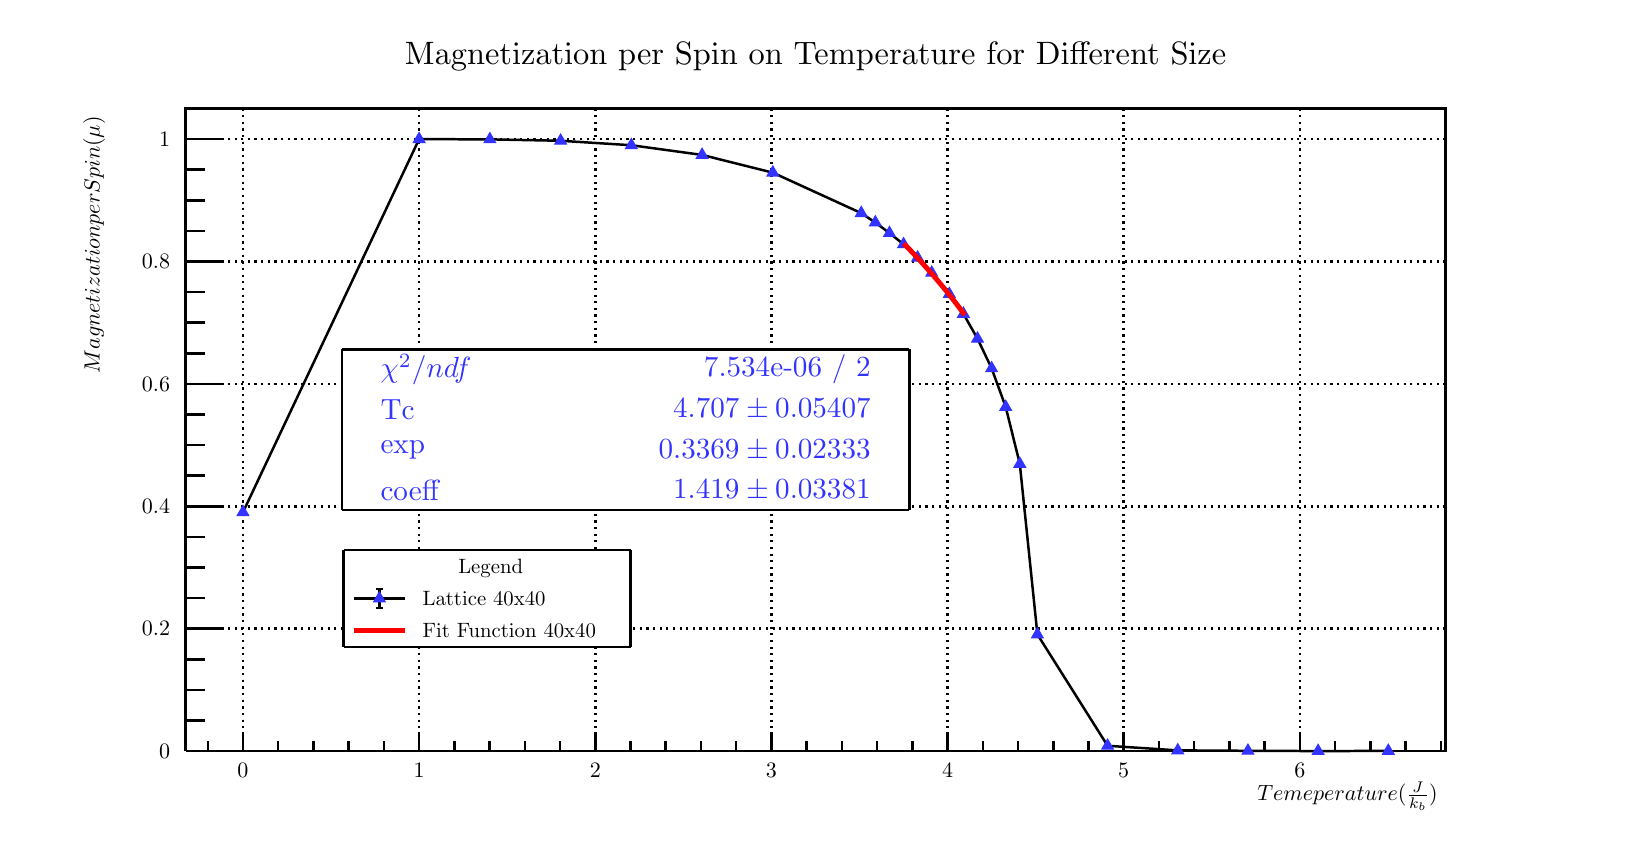
\begin{tikzpicture}
\pgfdeclareplotmark{cross} {
\pgfpathmoveto{\pgfpoint{-0.3\pgfplotmarksize}{\pgfplotmarksize}}
\pgfpathlineto{\pgfpoint{+0.3\pgfplotmarksize}{\pgfplotmarksize}}
\pgfpathlineto{\pgfpoint{+0.3\pgfplotmarksize}{0.3\pgfplotmarksize}}
\pgfpathlineto{\pgfpoint{+1\pgfplotmarksize}{0.3\pgfplotmarksize}}
\pgfpathlineto{\pgfpoint{+1\pgfplotmarksize}{-0.3\pgfplotmarksize}}
\pgfpathlineto{\pgfpoint{+0.3\pgfplotmarksize}{-0.3\pgfplotmarksize}}
\pgfpathlineto{\pgfpoint{+0.3\pgfplotmarksize}{-1.\pgfplotmarksize}}
\pgfpathlineto{\pgfpoint{-0.3\pgfplotmarksize}{-1.\pgfplotmarksize}}
\pgfpathlineto{\pgfpoint{-0.3\pgfplotmarksize}{-0.3\pgfplotmarksize}}
\pgfpathlineto{\pgfpoint{-1.\pgfplotmarksize}{-0.3\pgfplotmarksize}}
\pgfpathlineto{\pgfpoint{-1.\pgfplotmarksize}{0.3\pgfplotmarksize}}
\pgfpathlineto{\pgfpoint{-0.3\pgfplotmarksize}{0.3\pgfplotmarksize}}
\pgfpathclose
\pgfusepathqstroke
}
\pgfdeclareplotmark{cross*} {
\pgfpathmoveto{\pgfpoint{-0.3\pgfplotmarksize}{\pgfplotmarksize}}
\pgfpathlineto{\pgfpoint{+0.3\pgfplotmarksize}{\pgfplotmarksize}}
\pgfpathlineto{\pgfpoint{+0.3\pgfplotmarksize}{0.3\pgfplotmarksize}}
\pgfpathlineto{\pgfpoint{+1\pgfplotmarksize}{0.3\pgfplotmarksize}}
\pgfpathlineto{\pgfpoint{+1\pgfplotmarksize}{-0.3\pgfplotmarksize}}
\pgfpathlineto{\pgfpoint{+0.3\pgfplotmarksize}{-0.3\pgfplotmarksize}}
\pgfpathlineto{\pgfpoint{+0.3\pgfplotmarksize}{-1.\pgfplotmarksize}}
\pgfpathlineto{\pgfpoint{-0.3\pgfplotmarksize}{-1.\pgfplotmarksize}}
\pgfpathlineto{\pgfpoint{-0.3\pgfplotmarksize}{-0.3\pgfplotmarksize}}
\pgfpathlineto{\pgfpoint{-1.\pgfplotmarksize}{-0.3\pgfplotmarksize}}
\pgfpathlineto{\pgfpoint{-1.\pgfplotmarksize}{0.3\pgfplotmarksize}}
\pgfpathlineto{\pgfpoint{-0.3\pgfplotmarksize}{0.3\pgfplotmarksize}}
\pgfpathclose
\pgfusepathqfillstroke
}
\pgfdeclareplotmark{newstar} {
\pgfpathmoveto{\pgfqpoint{0pt}{\pgfplotmarksize}}
\pgfpathlineto{\pgfqpointpolar{44}{0.5\pgfplotmarksize}}
\pgfpathlineto{\pgfqpointpolar{18}{\pgfplotmarksize}}
\pgfpathlineto{\pgfqpointpolar{-20}{0.5\pgfplotmarksize}}
\pgfpathlineto{\pgfqpointpolar{-54}{\pgfplotmarksize}}
\pgfpathlineto{\pgfqpointpolar{-90}{0.5\pgfplotmarksize}}
\pgfpathlineto{\pgfqpointpolar{234}{\pgfplotmarksize}}
\pgfpathlineto{\pgfqpointpolar{198}{0.5\pgfplotmarksize}}
\pgfpathlineto{\pgfqpointpolar{162}{\pgfplotmarksize}}
\pgfpathlineto{\pgfqpointpolar{134}{0.5\pgfplotmarksize}}
\pgfpathclose
\pgfusepathqstroke
}
\pgfdeclareplotmark{newstar*} {
\pgfpathmoveto{\pgfqpoint{0pt}{\pgfplotmarksize}}
\pgfpathlineto{\pgfqpointpolar{44}{0.5\pgfplotmarksize}}
\pgfpathlineto{\pgfqpointpolar{18}{\pgfplotmarksize}}
\pgfpathlineto{\pgfqpointpolar{-20}{0.5\pgfplotmarksize}}
\pgfpathlineto{\pgfqpointpolar{-54}{\pgfplotmarksize}}
\pgfpathlineto{\pgfqpointpolar{-90}{0.5\pgfplotmarksize}}
\pgfpathlineto{\pgfqpointpolar{234}{\pgfplotmarksize}}
\pgfpathlineto{\pgfqpointpolar{198}{0.5\pgfplotmarksize}}
\pgfpathlineto{\pgfqpointpolar{162}{\pgfplotmarksize}}
\pgfpathlineto{\pgfqpointpolar{134}{0.5\pgfplotmarksize}}
\pgfpathclose
\pgfusepathqfillstroke
}
\definecolor{c}{rgb}{1,1,1};
\draw [color=c, fill=c] (0,0) rectangle (20,10.2002);
\draw [color=c, fill=c] (2,1.02002) rectangle (18,9.18019);
\definecolor{c}{rgb}{0,0,0};
\draw [c,line width=0.9] (2,1.02002) -- (2,9.18019) -- (18,9.18019) -- (18,1.02002) -- (2,1.02002);
\definecolor{c}{rgb}{1,1,1};
\draw [color=c, fill=c] (2,1.02002) rectangle (18,9.18019);
\definecolor{c}{rgb}{0,0,0};
\draw [c,line width=0.9] (2,1.02002) -- (2,9.18019) -- (18,9.18019) -- (18,1.02002) -- (2,1.02002);
\draw [c,line width=0.9] (2,1.02002) -- (18,1.02002);
\draw [c,dash pattern=on 0.80pt off 1.60pt ,line width=0.9] (2.72726,9.18019) -- (2.72726,1.02002);
\draw [c,dash pattern=on 0.80pt off 1.60pt ,line width=0.9] (4.96433,9.18019) -- (4.96433,1.02002);
\draw [c,dash pattern=on 0.80pt off 1.60pt ,line width=0.9] (7.2014,9.18019) -- (7.2014,1.02002);
\draw [c,dash pattern=on 0.80pt off 1.60pt ,line width=0.9] (9.43847,9.18019) -- (9.43847,1.02002);
\draw [c,dash pattern=on 0.80pt off 1.60pt ,line width=0.9] (11.6755,9.18019) -- (11.6755,1.02002);
\draw [c,dash pattern=on 0.80pt off 1.60pt ,line width=0.9] (13.9126,9.18019) -- (13.9126,1.02002);
\draw [c,dash pattern=on 0.80pt off 1.60pt ,line width=0.9] (16.1497,9.18019) -- (16.1497,1.02002);
\draw [c,dash pattern=on 0.80pt off 1.60pt ,line width=0.9] (2.72726,9.18019) -- (2.72726,1.02002);
\draw [c,dash pattern=on 0.80pt off 1.60pt ,line width=0.9] (16.1497,9.18019) -- (16.1497,1.02002);
\draw [c,line width=0.9] (2,1.02002) -- (2,9.18019);
\draw [c,dash pattern=on 0.80pt off 1.60pt ,line width=0.9] (18,1.02002) -- (2,1.02002);
\draw [c,dash pattern=on 0.80pt off 1.60pt ,line width=0.9] (18,2.57437) -- (2,2.57437);
\draw [c,dash pattern=on 0.80pt off 1.60pt ,line width=0.9] (18,4.12871) -- (2,4.12871);
\draw [c,dash pattern=on 0.80pt off 1.60pt ,line width=0.9] (18,5.68306) -- (2,5.68306);
\draw [c,dash pattern=on 0.80pt off 1.60pt ,line width=0.9] (18,7.23741) -- (2,7.23741);
\draw [c,dash pattern=on 0.80pt off 1.60pt ,line width=0.9] (18,8.79175) -- (2,8.79175);
\draw [c,dash pattern=on 0.80pt off 1.60pt ,line width=0.9] (18,8.79175) -- (2,8.79175);
\draw [c,line width=0.9] (2,1.02002) -- (18,1.02002);
\draw [c,line width=0.9] (2.72726,1.26483) -- (2.72726,1.02002);
\draw [c,line width=0.9] (3.17468,1.14242) -- (3.17468,1.02002);
\draw [c,line width=0.9] (3.62209,1.14242) -- (3.62209,1.02002);
\draw [c,line width=0.9] (4.0695,1.14242) -- (4.0695,1.02002);
\draw [c,line width=0.9] (4.51692,1.14242) -- (4.51692,1.02002);
\draw [c,line width=0.9] (4.96433,1.26483) -- (4.96433,1.02002);
\draw [c,line width=0.9] (5.41174,1.14242) -- (5.41174,1.02002);
\draw [c,line width=0.9] (5.85916,1.14242) -- (5.85916,1.02002);
\draw [c,line width=0.9] (6.30657,1.14242) -- (6.30657,1.02002);
\draw [c,line width=0.9] (6.75399,1.14242) -- (6.75399,1.02002);
\draw [c,line width=0.9] (7.2014,1.26483) -- (7.2014,1.02002);
\draw [c,line width=0.9] (7.64881,1.14242) -- (7.64881,1.02002);
\draw [c,line width=0.9] (8.09623,1.14242) -- (8.09623,1.02002);
\draw [c,line width=0.9] (8.54364,1.14242) -- (8.54364,1.02002);
\draw [c,line width=0.9] (8.99105,1.14242) -- (8.99105,1.02002);
\draw [c,line width=0.9] (9.43847,1.26483) -- (9.43847,1.02002);
\draw [c,line width=0.9] (9.88588,1.14242) -- (9.88588,1.02002);
\draw [c,line width=0.9] (10.3333,1.14242) -- (10.3333,1.02002);
\draw [c,line width=0.9] (10.7807,1.14242) -- (10.7807,1.02002);
\draw [c,line width=0.9] (11.2281,1.14242) -- (11.2281,1.02002);
\draw [c,line width=0.9] (11.6755,1.26483) -- (11.6755,1.02002);
\draw [c,line width=0.9] (12.123,1.14242) -- (12.123,1.02002);
\draw [c,line width=0.9] (12.5704,1.14242) -- (12.5704,1.02002);
\draw [c,line width=0.9] (13.0178,1.14242) -- (13.0178,1.02002);
\draw [c,line width=0.9] (13.4652,1.14242) -- (13.4652,1.02002);
\draw [c,line width=0.9] (13.9126,1.26483) -- (13.9126,1.02002);
\draw [c,line width=0.9] (14.36,1.14242) -- (14.36,1.02002);
\draw [c,line width=0.9] (14.8074,1.14242) -- (14.8074,1.02002);
\draw [c,line width=0.9] (15.2548,1.14242) -- (15.2548,1.02002);
\draw [c,line width=0.9] (15.7023,1.14242) -- (15.7023,1.02002);
\draw [c,line width=0.9] (16.1497,1.26483) -- (16.1497,1.02002);
\draw [c,line width=0.9] (2.72726,1.26483) -- (2.72726,1.02002);
\draw [c,line width=0.9] (2.27985,1.14242) -- (2.27985,1.02002);
\draw [c,line width=0.9] (16.1497,1.26483) -- (16.1497,1.02002);
\draw [c,line width=0.9] (16.5971,1.14242) -- (16.5971,1.02002);
\draw [c,line width=0.9] (17.0445,1.14242) -- (17.0445,1.02002);
\draw [c,line width=0.9] (17.4919,1.14242) -- (17.4919,1.02002);
\draw [c,line width=0.9] (17.9393,1.14242) -- (17.9393,1.02002);
\draw [anchor=base] (2.72726,0.683414) node[scale=0.795711, color=c, rotate=0]{0};
\draw [anchor=base] (4.96433,0.683414) node[scale=0.795711, color=c, rotate=0]{1};
\draw [anchor=base] (7.2014,0.683414) node[scale=0.795711, color=c, rotate=0]{2};
\draw [anchor=base] (9.43847,0.683414) node[scale=0.795711, color=c, rotate=0]{3};
\draw [anchor=base] (11.6755,0.683414) node[scale=0.795711, color=c, rotate=0]{4};
\draw [anchor=base] (13.9126,0.683414) node[scale=0.795711, color=c, rotate=0]{5};
\draw [anchor=base] (16.1497,0.683414) node[scale=0.795711, color=c, rotate=0]{6};
\draw [anchor= east] (18,0.448809) node[scale=0.795711, color=c, rotate=0]{$Temeperature (\frac{J}{k_{b}})$};
\draw [c,line width=0.9] (2,1.02002) -- (2,9.18019);
\draw [c,line width=0.9] (2.48,1.02002) -- (2,1.02002);
\draw [c,line width=0.9] (2.24,1.40861) -- (2,1.40861);
\draw [c,line width=0.9] (2.24,1.79719) -- (2,1.79719);
\draw [c,line width=0.9] (2.24,2.18578) -- (2,2.18578);
\draw [c,line width=0.9] (2.48,2.57437) -- (2,2.57437);
\draw [c,line width=0.9] (2.24,2.96295) -- (2,2.96295);
\draw [c,line width=0.9] (2.24,3.35154) -- (2,3.35154);
\draw [c,line width=0.9] (2.24,3.74013) -- (2,3.74013);
\draw [c,line width=0.9] (2.48,4.12871) -- (2,4.12871);
\draw [c,line width=0.9] (2.24,4.5173) -- (2,4.5173);
\draw [c,line width=0.9] (2.24,4.90589) -- (2,4.90589);
\draw [c,line width=0.9] (2.24,5.29447) -- (2,5.29447);
\draw [c,line width=0.9] (2.48,5.68306) -- (2,5.68306);
\draw [c,line width=0.9] (2.24,6.07165) -- (2,6.07165);
\draw [c,line width=0.9] (2.24,6.46023) -- (2,6.46023);
\draw [c,line width=0.9] (2.24,6.84882) -- (2,6.84882);
\draw [c,line width=0.9] (2.48,7.23741) -- (2,7.23741);
\draw [c,line width=0.9] (2.24,7.62599) -- (2,7.62599);
\draw [c,line width=0.9] (2.24,8.01458) -- (2,8.01458);
\draw [c,line width=0.9] (2.24,8.40317) -- (2,8.40317);
\draw [c,line width=0.9] (2.48,8.79175) -- (2,8.79175);
\draw [c,line width=0.9] (2.48,8.79175) -- (2,8.79175);
\draw [anchor= east] (1.9,1.02002) node[scale=0.795711, color=c, rotate=0]{0};
\draw [anchor= east] (1.9,2.57437) node[scale=0.795711, color=c, rotate=0]{0.2};
\draw [anchor= east] (1.9,4.12871) node[scale=0.795711, color=c, rotate=0]{0.4};
\draw [anchor= east] (1.9,5.68306) node[scale=0.795711, color=c, rotate=0]{0.6};
\draw [anchor= east] (1.9,7.23741) node[scale=0.795711, color=c, rotate=0]{0.8};
\draw [anchor= east] (1.9,8.79175) node[scale=0.795711, color=c, rotate=0]{1};
\draw [anchor= east] (0.836354,9.18019) node[scale=0.795711, color=c, rotate=90]{$Magnetization per Spin (\mu)$};
\definecolor{c}{rgb}{1,1,1};
\draw [color=c, fill=c] (3.98314,4.07897) rectangle (11.1907,6.12124);
\definecolor{c}{rgb}{0,0,0};
\draw [c,line width=0.9] (3.98314,4.07897) -- (11.1907,4.07897);
\draw [c,line width=0.9] (11.1907,4.07897) -- (11.1907,6.12124);
\draw [c,line width=0.9] (11.1907,6.12124) -- (3.98314,6.12124);
\draw [c,line width=0.9] (3.98314,6.12124) -- (3.98314,4.07897);
\definecolor{c}{rgb}{0.2,0.2,1};
\draw [anchor= west] (4.34352,5.86596) node[scale=1.05315, color=c, rotate=0]{$\chi^{2} / ndf $};
\draw [anchor= east] (10.8303,5.86596) node[scale=1.05315, color=c, rotate=0]{ 7.534e-06 / 2};
\draw [anchor= west] (4.34352,5.35539) node[scale=1.05315, color=c, rotate=0]{Tc       };
\draw [anchor= east] (10.8303,5.35539) node[scale=1.05315, color=c, rotate=0]{$ 4.707 \pm 0.05407$};
\draw [anchor= west] (4.34352,4.84482) node[scale=1.05315, color=c, rotate=0]{exp      };
\draw [anchor= east] (10.8303,4.84482) node[scale=1.05315, color=c, rotate=0]{$ 0.3369 \pm 0.02333$};
\draw [anchor= west] (4.34352,4.33425) node[scale=1.05315, color=c, rotate=0]{coeff    };
\draw [anchor= east] (10.8303,4.33425) node[scale=1.05315, color=c, rotate=0]{$ 1.419 \pm 0.03381$};
\definecolor{c}{rgb}{0,0,0};
\draw [c,line width=0.9] (2.72727,4.05307) -- (4.96434,8.79163) -- (5.86277,8.78873) -- (6.76121,8.77071) -- (7.65964,8.71413) -- (8.55807,8.59109) -- (9.4565,8.36566) -- (10.5795,7.85186) -- (10.7585,7.73291) -- (10.9375,7.59813) --
 (11.1164,7.45622) -- (11.2954,7.28581) -- (11.4744,7.09402) -- (11.6981,6.82364) -- (11.877,6.57233) -- (12.056,6.25693) -- (12.235,5.88052) -- (12.4139,5.39018) -- (12.5929,4.66736) -- (12.8166,2.5011) -- (13.7078,1.08727) -- (14.5991,1.02884) --
 (15.4903,1.02342) -- (16.3815,1.02002) -- (17.2727,1.02197);
\definecolor{c}{rgb}{0.2,0.2,1};
\foreach \P in {(2.72727,4.05307), (4.96434,8.79163), (5.86277,8.78873), (6.76121,8.77071), (7.65964,8.71413), (8.55807,8.59109), (9.4565,8.36566), (10.5795,7.85186), (10.7585,7.73291), (10.9375,7.59813), (11.1164,7.45622), (11.2954,7.28581),
 (11.4744,7.09402), (11.6981,6.82364), (11.877,6.57233), (12.056,6.25693), (12.235,5.88052), (12.4139,5.39018), (12.5929,4.66736), (12.8166,2.5011), (13.7078,1.08727), (14.5991,1.02884), (15.4903,1.02342), (16.3815,1.02053),
 (17.2727,1.02197)}{\draw[mark options={color=c,fill=c},mark size=2.402402pt,mark=triangle*] plot coordinates {\P};}
\definecolor{c}{rgb}{1,0,0};
\draw [c,line width=1.8] (11.1202,7.4645) -- (11.128,7.45654) -- (11.1358,7.44855) -- (11.1437,7.44055) -- (11.1515,7.43252) -- (11.1593,7.42448) -- (11.1672,7.41641) -- (11.175,7.40833) -- (11.1828,7.40022) -- (11.1907,7.3921) -- (11.1985,7.38395)
 -- (11.2063,7.37579) -- (11.2141,7.3676) -- (11.222,7.35939) -- (11.2298,7.35116) -- (11.2376,7.34291) -- (11.2455,7.33464) -- (11.2533,7.32635) -- (11.2611,7.31804) -- (11.269,7.3097) -- (11.2768,7.30135) -- (11.2846,7.29297) -- (11.2924,7.28457)
 -- (11.3003,7.27614) -- (11.3081,7.2677) -- (11.3159,7.25923) -- (11.3238,7.25074) -- (11.3316,7.24222) -- (11.3394,7.23369) -- (11.3472,7.22513) -- (11.3551,7.21654) -- (11.3629,7.20794) -- (11.3707,7.19931) -- (11.3786,7.19065) --
 (11.3864,7.18197) -- (11.3942,7.17327) -- (11.4021,7.16454) -- (11.4099,7.15579) -- (11.4177,7.14702) -- (11.4255,7.13822) -- (11.4334,7.12939) -- (11.4412,7.12054) -- (11.449,7.11167) -- (11.4569,7.10276) -- (11.4647,7.09384) -- (11.4725,7.08488)
 -- (11.4804,7.0759) -- (11.4882,7.0669) -- (11.496,7.05787) -- (11.5038,7.04881);
\draw [c,line width=1.8] (11.5038,7.04881) -- (11.5117,7.03972) -- (11.5195,7.03061) -- (11.5273,7.02147) -- (11.5352,7.0123) -- (11.543,7.00311) -- (11.5508,6.99389) -- (11.5587,6.98464) -- (11.5665,6.97536) -- (11.5743,6.96605) -- (11.5821,6.95671)
 -- (11.59,6.94735) -- (11.5978,6.93795) -- (11.6056,6.92853) -- (11.6135,6.91907) -- (11.6213,6.90959) -- (11.6291,6.90007) -- (11.6369,6.89053) -- (11.6448,6.88096) -- (11.6526,6.87135) -- (11.6604,6.86171) -- (11.6683,6.85204) -- (11.6761,6.84234)
 -- (11.6839,6.83261) -- (11.6918,6.82285) -- (11.6996,6.81305) -- (11.7074,6.80322) -- (11.7152,6.79336) -- (11.7231,6.78346) -- (11.7309,6.77353) -- (11.7387,6.76357) -- (11.7466,6.75357) -- (11.7544,6.74354) -- (11.7622,6.73348) --
 (11.7701,6.72338) -- (11.7779,6.71324) -- (11.7857,6.70307) -- (11.7935,6.69286) -- (11.8014,6.68261) -- (11.8092,6.67233) -- (11.817,6.66201) -- (11.8249,6.65166) -- (11.8327,6.64127) -- (11.8405,6.63084) -- (11.8484,6.62037) -- (11.8562,6.60986)
 -- (11.864,6.59931) -- (11.8718,6.58872) -- (11.8797,6.5781) -- (11.8875,6.56743);
\draw [c,line width=1.8] (11.8875,6.56743) -- (11.8953,6.55673);
\definecolor{c}{rgb}{1,1,1};
\draw [color=c, fill=c] (3.98314,4.07897) rectangle (11.1907,6.12124);
\definecolor{c}{rgb}{0,0,0};
\draw [c,line width=0.9] (3.98314,4.07897) -- (11.1907,4.07897);
\draw [c,line width=0.9] (11.1907,4.07897) -- (11.1907,6.12124);
\draw [c,line width=0.9] (11.1907,6.12124) -- (3.98314,6.12124);
\draw [c,line width=0.9] (3.98314,6.12124) -- (3.98314,4.07897);
\definecolor{c}{rgb}{0.2,0.2,1};
\draw [anchor= west] (4.34352,5.86596) node[scale=1.05315, color=c, rotate=0]{$\chi^{2} / ndf $};
\draw [anchor= east] (10.8303,5.86596) node[scale=1.05315, color=c, rotate=0]{ 7.534e-06 / 2};
\draw [anchor= west] (4.34352,5.35539) node[scale=1.05315, color=c, rotate=0]{Tc       };
\draw [anchor= east] (10.8303,5.35539) node[scale=1.05315, color=c, rotate=0]{$ 4.707 \pm 0.05407$};
\draw [anchor= west] (4.34352,4.84482) node[scale=1.05315, color=c, rotate=0]{exp      };
\draw [anchor= east] (10.8303,4.84482) node[scale=1.05315, color=c, rotate=0]{$ 0.3369 \pm 0.02333$};
\draw [anchor= west] (4.34352,4.33425) node[scale=1.05315, color=c, rotate=0]{coeff    };
\draw [anchor= east] (10.8303,4.33425) node[scale=1.05315, color=c, rotate=0]{$ 1.419 \pm 0.03381$};
\definecolor{c}{rgb}{0,0,0};
\draw (10,9.83933) node[scale=1.17016, color=c, rotate=0]{Magnetization per Spin on Temperature for Different Size};
\definecolor{c}{rgb}{1,1,1};
\draw [color=c, fill=c] (4.00421,2.34359) rectangle (7.65016,3.57119);
\definecolor{c}{rgb}{0,0,0};
\draw [c,line width=0.9] (4.00421,2.34359) -- (7.65016,2.34359);
\draw [c,line width=0.9] (7.65016,2.34359) -- (7.65016,3.57119);
\draw [c,line width=0.9] (7.65016,3.57119) -- (4.00421,3.57119);
\draw [c,line width=0.9] (4.00421,3.57119) -- (4.00421,2.34359);
\draw [anchor=base] (5.87276,3.27452) node[scale=0.748905, color=c, rotate=0]{Legend};
\draw [anchor=base west] (4.9157,2.86532) node[scale=0.748905, color=c, rotate=0]{Lattice 40x40};
\draw [c,line width=0.9] (4.14094,2.95739) -- (4.77898,2.95739);
\draw [c,line width=0.9] (4.45996,2.99954) -- (4.45996,3.08015);
\draw [c,line width=0.9] (4.45996,2.91524) -- (4.45996,2.83463);
\draw [c,line width=0.9] (4.41211,3.08015) -- (4.50781,3.08015);
\draw [c,line width=0.9] (4.41211,2.83463) -- (4.50781,2.83463);
\definecolor{c}{rgb}{0.2,0.2,1};
\foreach \P in {(4.45996,2.95739)}{\draw[mark options={color=c,fill=c},mark size=2.402402pt,mark=triangle*] plot coordinates {\P};}
\definecolor{c}{rgb}{0,0,0};
\draw [anchor=base west] (4.9157,2.45612) node[scale=0.748905, color=c, rotate=0]{Fit Function 40x40};
\definecolor{c}{rgb}{1,0,0};
\draw [c,line width=1.8] (4.14094,2.54819) -- (4.77898,2.54819);
\end{tikzpicture}
